\documentclass[11pt]{article}
\usepackage{authblk}

\usepackage{algorithm}
\usepackage{algorithmic}
\usepackage{amsmath}
\usepackage{amssymb}
\usepackage{graphicx}

\graphicspath{ {figs/clustering/} }

\renewcommand{\algorithmicrequire}{\textbf{Input:}}
\renewcommand{\algorithmicensure}{\textbf{Output:}}
\newcommand{\lp}{\left(}
\newcommand{\rp}{\right)}
\newcommand{\lb}{\left\{}
\newcommand{\rb}{\right\}}
\newcommand{\Real}{\mathbb{R}}
\newcommand{\rmax}{r_{\text{max}}}

\newcommand{\cC}{{\cal C}}
\newcommand{\cN}{{\cal N}}
\newcommand{\cM}{{\cal M}}
\newcommand{\cX}{{\cal X}}
\newcommand{\tM}{{\overline{M}}}
\newcommand{\ze}{z^*}

\DeclareMathOperator*{\argmax}{arg\,max}
\DeclareMathOperator*{\argmin}{arg\,min}

\title{CNTree Hierarchical Clustering}

\author[1]{Oren Livne\thanks{olivne@ets.org}}
\author[2]{Achi Brandt\thanks{achi.brandt@weizmann.ac.il}}
\affil[1]{Educational Testing Service, Attn: MS-12, T-197, 660 Rosedale Road, Princeton, NJ 08540}
\affil[2]{Faculty of Mathematics and Computer Science, The Weizmann Institute of Science, 234 Herzl Street, Rehovot 7610001 Israel}
\date{\today}

\begin{document}
\maketitle

\begin{abstract}
A stepping stone towards building multilevel optimization solvers for neural network training is clustering gradients of weights or activations into groups, and for each gradient computing a set of $p$ approximate nearest neighboring groups to interpolate from. This can be cast as the problem of clustering $n$ points in $\Real^m$ into $\sim n/3-n/2$ groups of small bounded radius (``mini-clustering'').

We present CNTree (Cluster and Neighbor Tree), an $O(m p n \log n)$ top-down hierarchical clustering algorithm that produces both groups and neighborhoods. The tree consists of levels of groups. Each group is split into $b$ subgroups at the next level. At each level of the tree we keep track of the neighbors of each group, which allows for an efficient application of local and global k-means iterations to determine  subgroup assignment and center locations.

In addition to inertia for measuring group quality, we define a neighborhood quality metric called ED (Excess Distance). Numerical experiments show that CNTree neighborhoods are exact in over $98\%$ of cases. A python implementation clusters $10^6$ points in $16$ dimensions in $3$ minutes on a single CPU.
\end{abstract}

\section{The Problem; Notation}
We consider the problem of clustering a set of $n$ points $\cX := \lb x_1\,\dots,x_n \rb $ in $\Real^m$ into $k$ small groups $\cC :=\lb C_1,\dots,C_k\rb $ (i.e., a coarsening ratio of $k/n \sim 0.3-0.2$). For simplicity, groups are non-overlapping. A {\it group} $C$ consists of a subset of $X$ and a {\it center}
\begin{equation}
	z(C) := \frac{1}{|C|}\sum_{x \in C} x\,.
\end{equation}
Points belonging to a group are called its {\it members}. Conversely, the $label(i)$ of a point $i$ is the group it belongs to. Instead of explicitly controlling the number of groups as in the standard k-means algorithm \cite{Lloyd82leastsquares} or the group size, we require that all groups have {\it radius} $r(C_j) \leq \rmax$, $j=1,\dots,k$, where
\begin{equation}
	r(C) := \lp \sum_{x \in C} \|x - z(C)\|^q \rp^{\frac{1}{q}}
\end{equation}
with a large enough $q$ so that the largest distances from the center dominate the sum; we use $q=4$.
The {\it distance measure} is the Euclidean distance $\|x-y\|$, although our algorithm works with any inner-product-induced norm.

For each $x_i, i=1,\dots,n$ we would also like to produce a {\it neighborhood}: a subset $N_i \subseteq \cC$ of $p$ approximately-nearest neighboring group centers, $z_j := z(C_j)$, $j=1,\dots,p$.

Given a (tentative neighbor) set $N$, $r_p(N,x) \subseteq N$ denotes the set of $p$ nearest neighors of $x$ in $N$.

\section{CNTree Algorithm}
Our algorithm is called CNTree (Clusters and Neighbors Tree), a top-down hierarchical clustering. The tree consists of $L$ increasingly-finer levels. Each level $l$, $l=1,\dots,L$, contains 
\begin{itemize}
	\item Groups $\cC^l := \lb C^l_1,\dots,C^l_{m_l}\rb$.
	\item Point neighborhoods $\cN^l := \lb N^l_1,\dots,N^l_n\rb $, i.e. the $p$ nearest neighboring group centers of each point.
	\item Group neighborhoods $\cM^l := \lb M^l_1,\dots,M^l_{m_l}\rb$, i.e. the $p$ nearest neighboring group center of each center (including itself: $j \in M^l_j$, $j=1,\dots,m_l$).
\end{itemize}

Level $1$ consists of a single group ($m_l=1$) containing all points, $M^1_1 = \lb 1\rb $ and $N^1_i = \lb 1\rb $, $j=1,\dots,n$. It is refined in $L$ stages until no group radius exceeds $\rmax$, so level $L$ is the final clustering result. 

Let $b \geq 2$ be the tree branching factor. We describe a refinement stage $l-1 \rightarrow l$. Level $l-1$ is the ``parent level'' and $l$ is the ``child level''.

For each $j=1,\dots,m^{l-1}$, we split the parent group $C^{l-1}_j$ into $b^{l-1}_j$ child groups, where
\begin{equation}
	b^{l-1}_j := 
	\begin{cases}
		b\,, &\mbox{if } r(C_j) > \rmax \text{ and } |C_j| \geq b\,, \\ 
		2\,, &\mbox{if } r(C_j) > \rmax \text{ and } |C_j| < b \,, \\ 
		1\,, &\mbox{otherwise.}
    \end{cases}
    \label{kj}
\end{equation}
Thus $m^l = \sum_{j=1}^{m^{l-1}} b^{l-1}_j$. We denote by $S^{l-1}_j$ the children set of $C^{l-1}_j$ and $parent^{l-1}(k)$ the parent of child $k$ (i.e., $parent(k) = j\, \forall k \in S_j$).

Children centers $\lb z^l_k \rb_{k \in S_j}$ are initialized to $b^{l-1}_j$ distinct random members of $C^{l-1}_j$ (better starts are conceivable but haven't been implemented, e.g., choose centers as points that are farthest from each other along the longest-axis dimension of the group).

The centers are first improved by $\nu_1$ relatively inexpensive local k-means iterations within each parent. That is, for each $j=1,\dots,m^{l-1}$ we set
\begin{equation}
	label^l(i) \leftarrow \argmin_{k \in S^{l-1}_i} \left\| x_i - z^l_k\right\|\,,\quad i \in C^{l-1}_j \,,
	\label{label_local}
\end{equation}
followed by updating child centers by
\begin{equation}
	z^l_k \leftarrow \frac{1}{|C^l_k|+1} \lp \sum_{x \in C^l_k} x + z^l_k \rp\,,\quad i \in C^{l-1}_j\,.
	\label{pakhira_local}
\end{equation}
Eq.~(\ref{pakhira_local}) was suggested by \cite{pakhira} to avoid empty groups, which are likely at the finest tree levels. This update also makes the k-means process more stable when a point is at nearly the same distance from multiple centers.

Subsequently, we perform $\nu_2$ iterations to globally improve the centers. In each iteration, we define the {\it tentative neighborhood} of child $k$ as
\begin{equation}
	\tilde{M}^l_k := \bigcup_{j' \in N_{parent(k)}} S_{j'}\,,
	\label{cousins}
\end{equation}
which the set of $k$'s siblings and cousins,
\begin{equation}
	M^l_k := r_p \lp z^l_k, \tilde{M}^l_k \rp\,.
\end{equation}
Similarly, we define point neighboorhoods by
\begin{equation}
	N^l_i := r_p \lp x_i, \tilde{M}^l_{label^l(i)} \rp\,,\quad i=1,\dots,n\,,
\end{equation}
$label^l(i)$ is $i$'s label at level $l$, i.e., the index $k$ of the child group $C^l_k$ it belongs to.

Next, we perform a global k-means iteration based on the constructed neighborhoods. Namely, each point is assigned to the nearest child center in its neighorhood:
\begin{equation}
	label^l(i) \leftarrow \argmin_{k \in N^l_{label^l(i)}} \left\| x_i - z^l_k\right\|\,,\quad i = 1,\dots,n\,,
	\label{label_global}
\end{equation}
followed by updating child centers by
\begin{equation}
	z^l_k \leftarrow \frac{1}{|C^l_k|+1} \lp \sum_{x \in C^l_k} x + z^l_k \rp\,,\quad i = 1,\dots,m^l\,.
	\label{pakhira_global}
\end{equation}
After $\nu_2$ global iterations, we recalculate point and child neighborhoods based on the new centers. This was shown to important to improve neighborhood quality for small $\nu_2$. We use $\nu_1=\nu_2=1$, since neighborhood quality seemed to only marginally improve by additional iterations.

\subsection{Optimized Distance Computation}
\label{distance}
A standard trick is to express
\begin{equation}
	\|x - y\|^2 = \langle x, x \rangle - 2 \langle x, y \rangle + \langle y, y \rangle
\end{equation}
so that  (\ref{label_global}) is equivalent to
\begin{equation}
	label^l(i) \leftarrow \argmin_{k \in N^l_{label^l(i)}} \lb  -2 \langle x_i, z^l_k \rangle + \langle z^l_k, z^l_k \rangle  \rb,,\quad i = 1,\dots,n\,,
	\label{label2}
\end{equation}
(\ref{label2}) is typically 2-3 times faster to evaluate than (\ref{label_global}), since the Python Numpy library inner product is highly optimized via vectorization.

\subsection{Stopping Criterion}
\label{stopping}
It turns out that insisting on all groups being smaller than the maximum radius is too restrictive. A more robust stopping criterion is
\begin{equation}
	\max \lb p_{90}\lp\lb C_j^l \rb_j\rp, \max_j \lp r(C_j^l) \rp / 1.5 \rb < \rmax\,,
	\label{stop}
\end{equation}
where $p_{90}$ is the $90${\it th} percentile of the radius distribution. In other words, once $90\%$ of the distribution is within $\rmax$, we allow the max radius to be up to $1.5 \rmax$. Since there's typically a small number of larger radius compared with the population, this allows us to reduce $L$ a little bit, and therefore the complexity.

\subsection{Small Groups}
\label{small}
If there are empty groups arise, they are removed at the end of the refinement stage, and deleted from all neighborhoods. This means that a small fraction of neighorhoods are potentially smaller, but since $p$ is increased by some number to start with (cf.~Sec.~\ref{neighborhood_size} below), we still get full neighborhoods for all points.

Furthermore, at the end of level processing, groups of size $1$ may have a non-zero radius because the center are not exactly aligned with the sole member due to the update (\ref{pakhira_global}). It is important to fix those centers to be the member coordinate so these groups are not considered for further refinement, as refinement is based on a radius threshold.

\subsection{Pseudo-Code}
In the pseudo code below, the data is expressed as an $n \times m$ matrix whose rows are point coordinates. The groups in $C^l$ are maintained both as sets $C^l_j$ and via $\{label^l(i)\}_i$ (the reverse mapping of point to group index).

\begin{algorithm}
\caption{CNTree}
\label{alg1}
\begin{algorithmic}[1]
\REQUIRE points $X_{n \times m}$; maximum group radius $\rmax$; branching factor $b$; neighorhood size $p$
\ENSURE groups $\cC^L$; neighborhoods $\cN^L$
\STATE $p \leftarrow p+2$
\STATE $l \leftarrow 1, \cC^l \leftarrow \lb\lb 1,\dots,n\rb \rb, M^l = \lb \lb 1 \rb \rb, N^l_i = \lb 1 \rb $, $j=1,\dots,n$
\WHILE{(\ref{stop}) doesn't hold}
	\STATE $l \leftarrow l+1$
	\FORALL{$j = 1,\dots,m^{l-1}$}
		\STATE Calculate $b^{l-1}_j$ by (\ref{kj})
		\STATE Initialize child centers of $C^{l-1}_j$ to $b^{l-1}_j$ distinct random members
	\ENDFOR
	\FORALL{$t=1,\dots,\nu_1$}
		\STATE Update labels within the parent (local k-means) by (\ref{label_local})
		\STATE Update child centers by (\ref{pakhira_local})
	\ENDFOR
 	\FORALL{$t=1,\dots,\nu_2+1$}
		\FORALL{$j = 1,\dots,m^l$}
			\STATE Calculate tentative group neighborhood $\tilde{M}^l_k \leftarrow \bigcup_{j' \in N_{parent(k)}} S_{j'}$
		\ENDFOR
		\IF{$t \leq \nu_2$}
			\FORALL{$j = 1,\dots,m^l$}
				\STATE Calculate group neighborhood $M^l_k \leftarrow r_p\lp z^l_k, \tilde{M}^l_k \rp$
			\ENDFOR
			\FORALL{$i = 1,\dots,n$}
				\STATE Calculate point neighborhood $N^l_i \leftarrow r_p\lp x_i, \tilde{M}^l_{label^l(i)} \rp$
			\ENDFOR
		\ENDIF
		\STATE Update point assignment (global k-means) by (\ref{label_global})
		\STATE Update child centers by (\ref{pakhira_global})
	\ENDFOR
	\STATE Remove empty groups from $\cC^L, \cM^L, \cN^L$.
	\STATE Set level $l$ centers of groups of size $1$ to their point coordinates.
\ENDWHILE
\end{algorithmic}
\end{algorithm}

\subsection{Complexity and Parameter Optimization}

\subsubsection{Neighorhood Size}
\label{neighborhood_size}
We work with neighboorhood size $p+2$ at all levels where $p$ is the target neighboorhood size in the final clustering. This is motivated by two reasons:
\begin{itemize}
	\item[(a)] Neighorhood accuracy boosting: it is possible to miss a nearest neighbor of child $k$ at level $l$ if $k$'s parent has many proximal neighbors. If the neighbor happens to be a child of a close neighbor of the parent that's however not among the parent's $p$ nearest neighbors, it won't be included in $\tilde{M}^l_k$. Since neighborhood accuracy (measured by mean and max ED, cf.~Sec.~\ref{metrics}) seems to increase exponentially with $p$, increasing $p$ by a small number increases accuracy without incurring a lot more work.
	\item[(b)] Empty group mitigation: after removing empty groups (cf.~Sec.~\ref{small}), some neighorhood sizes become smaller than $p$, so increasing $p$ initially restores them to be large enough.
\end{itemize}	


\subsubsection{Branching Factor}
i.e., the $p$ nearest neighboring groups of each group (including itselfThe worst-case complexity occurs when the points are distributed approximately uniformly (otherwise larger admissible groups can be formed in locally dense areas, hence the tree would have less levels and/or most groups in higher tree levels would be considered small and require no further splitting, reducing run-time). Here $L \approx \log_b n$, and level $l$ contains about $m_l=b^l$ groups. Level $l$ neighorhood construction requires $O(p b)$ distance computations per group and $O(p b)$ per point. Labels update requires $O(p)$ distance computations per point, and centers update requires $O(1)$ operations per point (amortized). Thus the dominating step is point neighorhood construction, and the total complexity is $O(\nu_2 b m p n \log_b n) = O(\nu_2 (b/\log_2 b) m p n \log_2 n)$. The term $b/\log_2 b$ is minimized for $b=e$, so the optimal $b$ is expected to be small (say, $2 \leq b \leq 4$). We didn't attempt to optimize $b$ and for simplicity (and to avoid the corner case of a larger number of empty groups, which is a bit problematic in our implementation) use $b=2$.

\section{Quality Metrics}
\label{metrics}
There exist plenty of clustering quality metrics \cite[Sec.~2.3.9]{sklearn_clustering}, however we need to properly interpret their value, as our data set does not have a small number of well-separated groups; we just wish to have reasonably separated groups. A simple metric is the {\it silhouette coefficient}. For each point we calculate the mean distance $a$ between the point and all other points in its group, and the mean distance $b$ between the point and all other points in the next nearest group. The silhouette coefficient is the mean of $(b-a)/\max\lb a,b \rb$ over all points. The score is in $[-1,1]$ and is higher when groups are dense and well separated. It does not require knowing the true labels, which are anyway fuzzy in this case. A silhouette coefficient of $0.3-0.5$ is good enough for our purposes.

To measure neighboorhood quality, we calculate the exact $p$ nearest neighboring groups $\ze_{i,1},\dots,\ze_{i,p}$ of each point $i$ by brute force. Let $N_i = \left\{z_{i,1},\dots,z_{i,p}\rb $ be the neighorhood of point $i$ (sorted by ascending distance from $x_i$). We measure
\begin{equation}
	\text{ED}_{t,i} := \frac{\|z_{i,t} - x_i\| - \|\ze_{i,t} - x_i\|}{\|\ze_{i,t} - x_i\|}\,\qquad i=1,\dots,n\,, t=1,\dots,p\,.
\end{equation}
$ED_{t,i}$ is the Excess Distance (MED) of the $t${\it th} approximate nearest neighbor relative to the true $t${\it th} nearest neighbor for point $i$. $ED_{t,i} = 0$ means point $i$'s neighborhood includes the $t${\it th} the nearest neighbor; $ED_{t,i}=1$ means the approximate $t${\it th} neighbor is twice as far as the true one; and so on. Useful statistics are the mean, median and max ED over all points. 

\section{Results}
CNTree was implemented in Python, and the low-level routines were optimized with Cython. All reported experiments were run on a single Intel Xeon CPU, 3.2GHz, 64-bit Ubuntu machine with $p=5$, since that's a typical neighrhood size for interpolation construction.

\subsection{Random Points}
We generated $n$ random points in $[0,1]^m$ and measured the ED statistics as a function of $n$. The maximum group radius was $\rmax = 1.5 n^{-1/m}$, which is equivalent to a roughly constant coarsening ratio $\rho := |\cC^L|/n$, because the expected number of points within a ball of radius $r$ in $\Real^m$ is $n V_m r^m$, where $V_m$ is the volume of the $n$-dimensional unit ball.

\begin{table}
\begin{tabular}{l*{6}{c}r}
	$m \times n$ & $\rho$ & Stat & Nbhr $1$ & Nbhr $2$ & Nbhr $3$ & Nbhr $4$ & Nbhr $5$ \\
	\hline
	\hline
	$1000 \times 2$		& 0.25  & mean   & 0.31 & 1.32 &  1.65 & 2.18 & 2.96 \\
	                    &       & median & 0    & 0    &  0    & 0    & 0    \\
       	 		   	  	&       & max    & 217  & 147  &  111  & 89   & 62   \\
	\hline
	$10000 \times 2$	& 0.24  & mean   & 0.17 & 1.79 &  2.28 & 3.18 & 4.20 \\
	                    &       & median & 0    & 0    &  0    & 0    & 0    \\
       	 		   	  	&       & max    & 214  & 243  &  163  & 109  & 830  \\
	\hline
	$20000 \times 2$	& 0.24  & mean   & 0.22 & 2.27 &  2.48 & 3.32 & 4.71 \\
	                    &       & median & 0    & 0    &  0    & 0    & 0    \\
       	 		   	  	&       & max    & 484  & 1137 &  194  & 131  & 130  \\
	\hline
	\hline
	$1000 \times 8$		& 0.25  & mean   & 0.78 & 8.13 &  10.4 & 12.1 & 13.4 \\
	                    &       & median & 0    & 0    &  6.9  & 9.8  & 11.5 \\
       	 		   	  	&       & max    & 101  & 92   &  70   & 65   & 60   \\
	\hline
	$10000 \times 8$	& 0.24  & mean   & 1.32 & 13.9 &  15.6 & 17.6 & 20   \\
	                    &       & median & 0    & 6    &  11.9 & 15.1 & 18   \\
       	 		   	  	&       & max    & 115  & 147  &  115  & 109  & 98   \\
	\hline
	$20000 \times 8$	& 0.25  & mean   & 1.63 & 14.6 &  16.5 & 18.5 & 20.9 \\
	                    &       & median & 0    & 7    &  13   & 16   & 19   \\
       	 		   	  	&       & max    & 145  & 189  &  132  & 130  & 141  \\

	\end{tabular}
	\caption{Excess distance ($\%$) mean and max between points and neighboring clusters vs. number of points for the uniformly random experiment.}
	\label{ed_vs_size}
\end{table}

The median ED was $0$ for all neighbors $t$ and all $n$ for $m=2$, and is still very small ($ \leq 20\%$) for $m=8$. This means that for the vast majority of points our neighborhoods are almost exact and the bad cases are very unlikely. Fig..~\ref{ed_distribution} shows the ED distribution for the $n=50000$. Only $2\%$ have non-zero ED, $1\%$ have $ED > 1$, and $0.1\%$ have $ED > 2$. Even the mean ED stays fairly stable with $n$.

\begin{figure}[htbp]
	\begin{center}
	\begin{tabular}{c}
        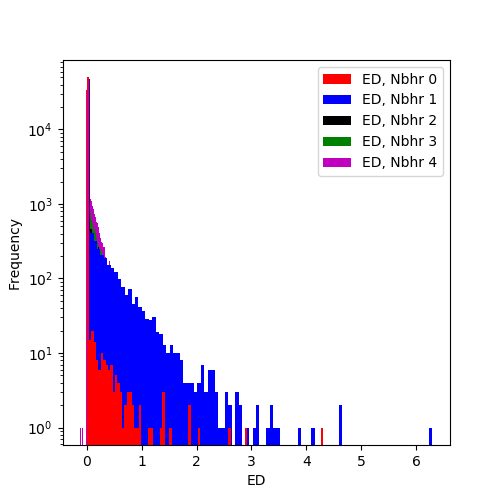
\includegraphics[width=0.7\textwidth]{ed_distribution} \\
    \end{tabular}
    \end{center}
	\label{ed_distribution}
	\caption{CNTree clustering for $n = 50000, m=2$. Top: uniformly random points in. Bottom: Gaussian mixture.}
\end{figure}

\subsection{Gaussian Mixture}
In this experiment we generated $1200$ points by mixing $12$ multivariate Gaussian distributions with standard deviation $\sigma=1$, whose means were on a $3 \times 3$ grid with spacing $d = 10 \sigma$ (easy, non-overlapping case) and $d=2\sigma$ (overlapping clusters). $100$ points were sampled from each distribution.

In this case we expect clusters to be accurately reproduced for large $d$. All clusters were correctly separated for $d=10\sigma$. However, due to the hierarhical, progressive nature of the algorithm, clusters can be split between intermediate level groups, leading to several clusters that were split into $2-3$ groups each in the final result; see Fig.~\ref{models}. For $d=2\sigma$ a lot more clusters ($88$) were identified, which is to be expected since the original $9$ clusters are not clearly separated.

\begin{figure}[htbp]
	\begin{center}
	\begin{tabular}{cc}
        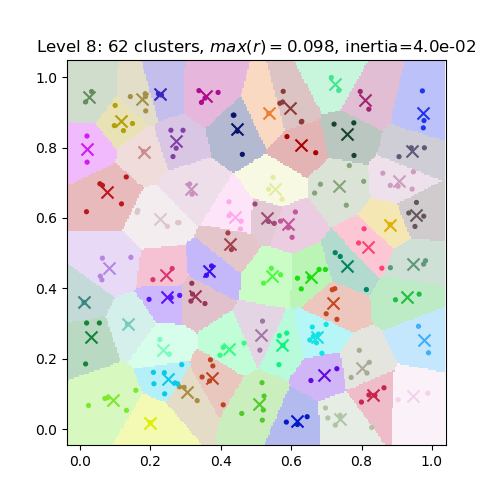
\includegraphics[width=0.45\textwidth]{clustering_uniform_200_r_01} &
        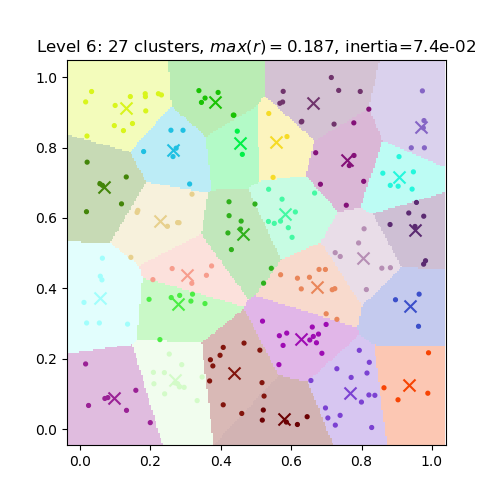
\includegraphics[width=0.45\textwidth]{clustering_uniform_200_r_02}
        \\
        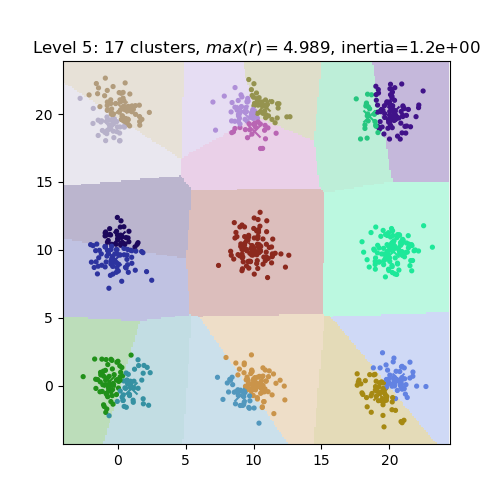
\includegraphics[width=0.45\textwidth]{clustering_gaussian_mixture_d_10} &
        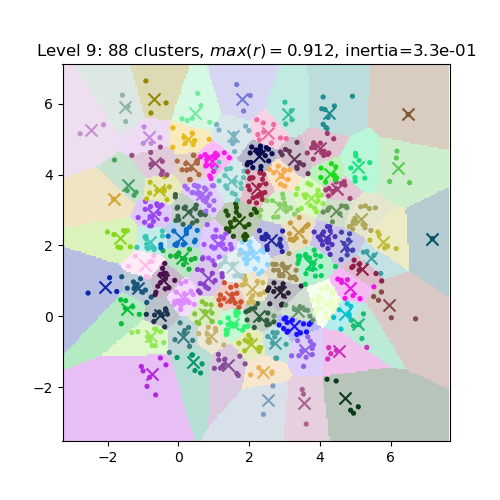
\includegraphics[width=0.45\textwidth]{clustering_gaussian_mixture_d_2}
    \end{tabular}
    \end{center}
	\label{models}
	\caption{CNTree clustering. Top: uniformly random points with $\rmax=0.1$ (left), $\rmax=0.2$ (right). Bottom: Gaussian mixture with $d=10 \sigma$ (left) and $d = 2\sigma$ (right).}
\end{figure}

\subsection{Runtime Scaling}
We tested $n$ uniformly distributed points in $\Real^m$ and measured the run-time.
\begin{table}
\begin{tabular}{l*{6}{c}r}
$n$ & $m = 2$ & $m = 4$ & $m = 8$ & $m = 16$ & $m = 32$ \\
\hline
\hline
$10^3$ & 0.121 & 0.085 & 0.095 & 0.229 & 0.38  \\
$10^4$ & 1.069 & 0.990 & 1.070 & 1.861 & 3.025 \\
$10^5$ & 8.76  & 8.240 & 12.5  & 21.9  & 38.2  \\ 
$10^6$ & 122   & 116   & 121   & 206   & -     \\ 
	\end{tabular}
	\caption{Runtimes [sec] vs. number of points $n$ and dimensions $m$.}
\end{table}
The runtime scales roughly linearly with $n$ and $m$. The time fluctuations can be partially explained by the fact that the coarsening ratio wasn't exactly constant, so the number of levels may have been relatively larger in some experiments than for others.

\subsection{Conclusion}
We presented a linear-scaling clustering scheme, CNTree, which also provides accurate nearest-neighborhoods. While further optimization can be implemented, the algorithm can already cluster $10^6$ points in $16$ dimensions in $3$ minutes, which should be good enough for our neural network training application.

\bibliography{msgd}
\bibliographystyle{plain}

\end{document}
